\chapter{Galaxies and the Motions of Stars}
\label{ch:galaxies}

A galaxy holds some $10^{11}$ stars with gas and dust between them, all bound by their own gravity. Galaxies in turn gather into groups and into clusters of hundreds or thousands. Seen from far enough away, each star in a galaxy and each galaxy in a cluster is a point that moves in the pull of all the others.

No new physics is needed to describe them. The gravity of a sphere (P2) and conservation of momentum (P1) turn the speed of an orbit into the mass inside it. The virial theorem of Chapter~\ref{ch:selfgrav} turns random speeds into a mass in the same way. The random walk (P5) decides whether the stars of a system ever trade energy among themselves. Applied to galaxies, these simple tools give a result nobody expected. Most of the mass sends out no light at all.

% ==============================================================================
\section{Our Galaxy}
\label{ga:sec:galaxy}

Chapter~\ref{ch:coords} set up Galactic coordinates on the band of the Milky Way (Section~\ref{co:sec:galactic}). Chapter~\ref{ch:ism} found the thin gas between the stars and the $21\,\mathrm{cm}$ line that traces it (Section~\ref{is:sec:21cm}).

Both say where things lie on the sky. Neither says how the Galaxy is built in depth, or how much it weighs. We sit inside a dusty disk and cannot step outside to look at it.

Throw a ball straight up. It climbs until gravity has taken away its speed, and then it falls back. Thrown at the same speed on the Moon, it climbs six times higher, because the Moon pulls six times more weakly. Without any scale, the height reached at a given speed weighs the body underneath.

The stars of the Galactic disk do the same. Each one bobs up and down through the plane as it circles the centre, at a few tens of kilometres per second. The disk pulls it back, and how far it rises before turning measures that pull. The pull of a wide flat layer is set by its mass per unit area. So the thickness of the disk weighs the disk.

The ball in symbols. Thrown at speed $v$ against the pull $g$, it rises to $v^2/2g$. That is $5.1\,\mathrm m$ for $10\,\mathrm{m\,s^{-1}}$ on the Earth and $31\,\mathrm m$ on the Moon, where $g=1.62\,\mathrm{m\,s^{-2}}$. Near the Sun the disk pulls with $g\approx6\times10^{-11}\,\mathrm{m\,s^{-2}}$ (below), so a star that crosses the plane at $20\,\mathrm{km\,s^{-1}}$ rises about $100\,\mathrm{pc}$ before it turns back.

The picture is the disk seen edge on, a thin bright layer with stars swinging through it like weights on springs. The faster ones reach further out.

The same balance is hydrostatic equilibrium (Section~\ref{sg:sec:hse}) for a gas made of stars. It is momentum conservation (P1) with the gravity of a flat layer from Gauss's law (P2). It sets the thickness of the gas around a young star, and it is how Oort first weighed the disk near the Sun. It gives the parts of the Galaxy, the mass at its centre, and the mass per unit area of its disk.

\paragraph{The parts.} The Galaxy has four parts, listed in Table~\ref{ga:tab:galaxy}. The \textbf{disk} holds most of the stars, nearly all the gas and dust, and the spiral arms where new stars form. The \textbf{bulge}, with a bar, fills the central few kiloparsecs with old stars. The \textbf{stellar halo} is a sparse round cloud of old stars poor in metals, with about $150$ globular clusters. The \textbf{dark halo} is known only from its pull (Section~\ref{ga:sec:rotation}), and it holds most of the mass. The Sun lies in the disk at $R_0=8.2\,\mathrm{kpc}$ from the centre, about $20\,\mathrm{pc}$ north of the plane, and it circles at $v_0\approx230\,\mathrm{km\,s^{-1}}$, the speed of the local standard of rest of Section~\ref{as:sec:uvw}.

\begin{table}[htbp]
	\centering
	\begin{tabular}{@{}l l l p{0.33\textwidth}@{}}
		\toprule
		\textbf{Part} & \textbf{Size} & \textbf{Mass} ($M_\odot$) & \textbf{Contents} \\
		\midrule
		Disk & scale length $2.6\,\mathrm{kpc}$, & stars $4\times10^{10}$, & young and old stars, gas, dust, \\
		 & thickness $0.3$ and $0.9\,\mathrm{kpc}$ & gas $1\times10^{10}$ & spiral arms \\
		Bulge and bar & central $2$--$3\,\mathrm{kpc}$ & $1.5\times10^{10}$ & old stars \\
		Stellar halo & out to $100\,\mathrm{kpc}$ and more & $1\times10^{9}$ & old metal-poor stars, globular clusters \\
		Dark halo & out to $200$--$300\,\mathrm{kpc}$ & $1\times10^{12}$ & unseen \\
		Central black hole & inside $120\,\mathrm{AU}$ & $4\times10^{6}$ & Sagittarius A* \\
		\bottomrule
	\end{tabular}
	\caption{The parts of the Milky Way, with rounded sizes and masses. The disk has a thin and a thick component.}
	\label{ga:tab:galaxy}
\end{table}

The picture took a long time to find. Herschel and later Kapteyn counted stars in every direction and placed the Sun near the middle of a small flattened system. They did not know about dust. Extinction (Chapter~\ref{ch:photometry}) hides everything beyond a few kiloparsecs in the plane, so in every direction the counts saw the same nearby patch. Shapley used the globular clusters instead. They lie mostly out of the plane, above the dust, and they form a round swarm whose centre is far away in Sagittarius. That centre is the centre of the Galaxy. The $21\,\mathrm{cm}$ line passes through dust and maps the gas over the whole disk. Infrared light also passes through, and shows the bulge.

\paragraph{The mass at the centre.} The radio source Sagittarius A* sits at the zero point of Galactic coordinates (Section~\ref{co:sec:galactic}). Stars close to it move on Kepler orbits that infrared cameras have followed for decades. The star S2 has a period of $16.05$ years and a semi-major axis of $0.1255''$ on the sky. To weigh what it orbits, we use Kepler's third law $n^2a^3=GM$ (Eq.~\eqref{eq:kepler3}) with the mean motion $n=2\pi/P$ for a period $P$, and divide by the same law for the Earth round the Sun,
\begin{align}
	\frac{M}{M_\odot}
	&\eqby{1} \frac{(2\pi/P)^2\,a^3}{(2\pi/1\,\mathrm{yr})^2\,(1\,\mathrm{AU})^3}
	= \left(\frac{a}{1\,\mathrm{AU}}\right)^3\left(\frac{P}{1\,\mathrm{yr}}\right)^{-2} \nonumber\\
	&\eqby{2} \frac{(0.1255\times8180)^3}{16.05^2}
	= 4.2\times10^6 .
\end{align}
\begin{explain}
	\item Eq.~\eqref{eq:kepler3} for S2, divided by the same equation for the Earth, $GM_\odot=(2\pi/1\,\mathrm{yr})^2(1\,\mathrm{AU})^3$.
	\item An angle of $1''$ at $1\,\mathrm{pc}$ spans $1\,\mathrm{AU}$ (Eq.~\eqref{eq:parallax_def}), so $0.1255''$ at $8180\,\mathrm{pc}$ is $1027\,\mathrm{AU}$.
\end{explain}
S2 comes within $120\,\mathrm{AU}$ of the centre. Four million solar masses inside so small a region, giving out very little light, can only be a black hole. The same orbit fixes $R_0$ as well. The Doppler shift of S2 gives its speed in kilometres per second and its motion on the sky gives the same speed in seconds of arc per year, and their ratio is the distance, $8.18\,\mathrm{kpc}$.

\paragraph{The pull of a flat layer.} Near the Sun the disk is about $0.3\,\mathrm{kpc}$ thick and changes over a few kiloparsecs along the plane, so locally it is a wide flat layer. Let $\Sigma$ be its mass per unit area and let $z$ be the height above its middle. By symmetry the pull points toward the plane and depends only on $|z|$. Take a box of face area $A$ with faces at $+z$ and $-z$, both outside most of the layer, so that it holds the mass $\Sigma A$. Gauss's law \eqref{pr:eq:gauss_gravity} gives
\begin{align}
	-4\pi G\,\Sigma A
	&\eqby{1} \oint\vec g\cdot d\vec A \nonumber\\
	&\eqby{2} -g(z)\,A-g(z)\,A \nonumber\\
	\implies\quad g(z)
	&= 2\pi G\Sigma .
\end{align}
\begin{explain}
	\item Eq.~\eqref{pr:eq:gauss_gravity} with the mass $\Sigma A$ inside the box (P2).
	\item On the top face $\vec g$ points down and $d\vec A$ points up, and on the bottom face the reverse. On the sides $\vec g$ lies along the face and gives nothing.
\end{explain}
\begin{equation}
	\boxed{g=2\pi G\Sigma}
	\label{ga:eq:sheet_g}
\end{equation}
Above the layer the pull does not weaken with height, just as the field of a charged plane does not. For $\Sigma=70\,M_\odot\,\mathrm{pc^{-2}}$ it is $6.1\times10^{-11}\,\mathrm{m\,s^{-2}}$.

\paragraph{A gas of stars above the layer.} Now follow one population of stars, say old dwarfs of one type, with mass density $\rho(z)$, and let most of them lie above most of the layer's mass. Let $\sigma_z^2=\avg{v_z^2}$ be the mean square of their vertical speed at height $z$. The momentum flux \eqref{pr:eq:momentum_flux} counted the momentum that particles carry across a surface as they move through it. No collisions entered that count, so it holds for stars. Its $zz$ entry is $\rho\avg{v_z^2}=\rho\sigma_z^2$ when there is no mean vertical flow. In a steady flat layer only derivatives along $z$ survive, and the $z$ component of Eq.~\eqref{pr:eq:momentum_conservative} reads
\begin{align}
	0
	&\eqby{1} \pdv{(\rho\avg{v_z})}{t}+\dv{z}\Pi_{zz}-\rho\,g_z \nonumber\\
	&\eqby{2} \dv{z}\big(\rho\sigma_z^2\big)+2\pi G\Sigma\,\rho .
\end{align}
\begin{explain}
	\item Eq.~\eqref{pr:eq:momentum_conservative}, $z$ component, with no change along $x$ or $y$ (P1).
	\item No mean vertical motion and no change in time, $\Pi_{zz}=\rho\sigma_z^2$, and $g_z=-2\pi G\Sigma$ above the layer by Eq.~\eqref{ga:eq:sheet_g}.
\end{explain}
If $\sigma_z$ is the same at every height, this is $\dv*{\rho}{z}=-\rho/h_z$, and
\begin{equation}
	\boxed{\rho(z)\propto e^{-z/h_z},\qquad h_z=\frac{\sigma_z^2}{2\pi G\Sigma}.}
	\label{ga:eq:disk_height}
\end{equation}
This is the scale height of an atmosphere, Eq.~\eqref{sg:eq:scale_height}, with $k_BT/(\mu m_{\rm H})$ replaced by $\sigma_z^2$ and the surface gravity by $2\pi G\Sigma$. Stars with larger vertical speeds make a thicker layer, and a heavier disk makes a thinner one. For $\sigma_z=20\,\mathrm{km\,s^{-1}}$ and $\Sigma=70\,M_\odot\,\mathrm{pc^{-2}}$, $h_z=210\,\mathrm{pc}$, close to the $300\,\mathrm{pc}$ of the old thin disk.

\paragraph{Weighing the disk.} Turned around, $\Sigma=\sigma_z^2/(2\pi Gh_z)$. Counting stars of one type at increasing heights gives $h_z$, and their spectra give $\sigma_z$. Kuijken and Gilmore did this for about five hundred K dwarfs toward the south Galactic pole and found $\Sigma\approx70\,M_\odot\,\mathrm{pc^{-2}}$ within $1.1\,\mathrm{kpc}$ of the plane. The stars and gas that can be seen near the Sun add up to about $50\,M_\odot\,\mathrm{pc^{-2}}$. The difference is about what a round dark halo puts into a slab of that thickness (Problem~\ref{ga:prob:sun}). Near the Sun the dark matter is spread through the halo, not packed into the disk.

% ==============================================================================
\section{Rotation Curves and Dark Matter}
\label{ga:sec:rotation}

Chapter~\ref{ch:twobody} weighed the Sun from the orbits of its planets. The gravity of a sphere (P2, Eq.~\eqref{pr:eq:shell_theorem}) says that an extended body pulls as if the mass inside the orbit sat at the centre.

In a galaxy the mass is spread out over many kiloparsecs, and we do not know how. What we see is light, and light need not follow mass.

Think of the planets. Mercury moves at $47\,\mathrm{km\,s^{-1}}$, the Earth at $30$, Neptune at only $5.4$. Further out, the planets move slower, because all the mass that holds them is in the Sun at the middle. If Neptune moved as fast as the Earth, the mass inside its orbit would have to be thirty times the mass inside the Earth's orbit, and that extra mass would have to be somewhere between the two.

The stars and gas clouds of a spiral galaxy circle its centre in the same way. Their speed at each radius gives the mass inside that radius, whether that mass shines or not. Beyond the edge of the light, the speeds should fall as Neptune's do. They stay flat. The orbital speed weighs everything inside the orbit, seen or unseen.

The planets in symbols. A circular orbit at radius $r$ about a mass $M$ has $v^2=GM/r$, so $v\propto r^{-1/2}$, and Neptune at $30.07\,\mathrm{AU}$ moves at $29.78/\sqrt{30.07}=5.43\,\mathrm{km\,s^{-1}}$. The Sun moves round the Galaxy at $v_0=230\,\mathrm{km\,s^{-1}}$ at $R_0=8.2\,\mathrm{kpc}$, so the mass inside the Sun's orbit is $v_0^2R_0/G=1.0\times10^{11}\,M_\odot$. One lap takes $2\pi R_0/v_0=220$ million years.

The picture is Figure~\ref{ga:fig:rotation}. The speed rises steeply near the centre, then stays level far beyond the stars.

The same weighing finds the mass of the Earth from the Moon, of Jupiter from its moons, and of the black hole from S2. Here it is P2 with momentum conservation (P1) for a circle, and the flat curve is the isothermal sphere of Section~\ref{st:sec:polytropes}. In Chapter~\ref{ch:universe} the same unseen matter decides how galaxies form at all. It gives the circular speed in any round galaxy, how to measure it from inside our own, a model with a halo, and the mass-to-light ratio.

\paragraph{The circular speed.} To find the speed of a circular orbit at radius $r$ in any spherical distribution of mass, we equate the acceleration of the orbit with the pull of the mass inside,
\begin{align}
	-\frac{v_{\rm circ}^2}{r}\,\rhat
	&\eqby{1} \dv{\vec v}{t}
	\eqby{2} \vec g(r)
	\eqby{3} -\frac{G\,m(r)}{r^2}\,\rhat .
\end{align}
\begin{explain}
	\item Motion on a circle at constant speed $v_{\rm circ}$.
	\item A star moves under gravity alone (P1 for its momentum).
	\item The gravity of a sphere, Eq.~\eqref{pr:eq:shell_theorem} (P2).
\end{explain}
\begin{equation}
	\boxed{v_{\rm circ}^2=\frac{G\,m(r)}{r}.}
	\label{ga:eq:vcirc}
\end{equation}
The speed at $r$ depends only on the mass inside $r$, however it is arranged in radius, and the mass outside drops out. That holds exactly for a round halo. For a flat disk the mass outside $r$ also pulls, so for a disk the relation is only a good estimate. The graph of $v_{\rm circ}$ against $r$ is the \textbf{rotation curve}.

\paragraph{Reading a rotation curve.} Turned around, $m(r)=v_{\rm circ}^2r/G$. Each shape of the curve stands for one way of spreading the mass.
\begin{center}
	\begin{tabular}{@{}l l l@{}}
		\toprule
		\textbf{Mass} & $m(r)$ & $v_{\rm circ}$ \\
		\midrule
		all at the centre & constant & $\propto r^{-1/2}$ \\
		uniform sphere & $\propto r^3$ & $\propto r$ \\
		flat curve & $\propto r$ & constant \\
		\bottomrule
	\end{tabular}
\end{center}
For a flat curve the density follows from $\dv*{m}{r}=4\pi r^2\rho$,
\begin{align}
	\rho
	&\eqby{1} \frac{1}{4\pi r^2}\,\dv{m}{r}
	\eqby{2} \frac{1}{4\pi r^2}\,\dv{r}\left(\frac{v_{\rm circ}^2\,r}{G}\right)
	= \frac{v_{\rm circ}^2}{4\pi G\,r^2} .
\end{align}
\begin{explain}
	\item Eq.~\eqref{pr:eq:mass_inside}.
	\item Eq.~\eqref{ga:eq:vcirc} with $v_{\rm circ}$ the same at every radius.
\end{explain}
\begin{equation}
	\boxed{\rho=\frac{v_{\rm circ}^2}{4\pi G\,r^2}\qquad\text{(flat rotation curve)}.}
	\label{ga:eq:rho_flat}
\end{equation}
The isothermal sphere of Section~\ref{st:sec:polytropes} gives the same law by another route. Far from its centre it has $\rho=c_s^2/(2\pi Gr^2)$ and $v_{\rm circ}^2=2c_s^2$, and putting $c_s^2=v_{\rm circ}^2/2$ into the first gives Eq.~\eqref{ga:eq:rho_flat}. A flat rotation curve is what a halo of particles with one velocity spread at every radius produces.

\paragraph{Measuring the rotation from inside.} We see our own Galaxy from a point on one of its orbits. To get $v_{\rm circ}$ at other radii, we measure the Doppler shift of the $21\,\mathrm{cm}$ line at Galactic longitude $l$ in the plane, and work out what circular motion predicts for it.

Put the origin at the Galactic centre, with $\hat x$ from the Sun toward the centre ($l=0$), $\hat y$ toward $l=90^\circ$, the direction of rotation at the Sun, and $\hat z$ toward the north Galactic pole (Figure~\ref{ga:fig:tangent}). These are the axes of $(U,V,W)$ of Section~\ref{as:sec:uvw}, moved to the centre. The Sun is at $\vecr_0=(-R_0,\,0)$ in the plane. A cloud at distance $d$ along the direction of sight $\hat{\mathbf s}=(\cos l,\,\sin l)$ is at $\vecr=\vecr_0+d\,\hat{\mathbf s}$, at distance $r=|\vecr|$ from the centre. Seen from the north pole the Galaxy turns clockwise. A body on a circular orbit at $\vecr$ with angular speed $\omega(r)=v_{\rm circ}(r)/r$ therefore has the velocity
\begin{equation}
	\vec v=\omega(r)\,\mathbf J\,\vecr,\qquad
	\mathbf J=\begin{pmatrix}0&1\\-1&0\end{pmatrix},
\end{equation}
a turn of $\vecr$ by $-90^\circ$ scaled by $\omega$. At the Sun, $\mathbf J\vecr_0=(0,\,R_0)$, so $\vec v_0=\omega_0R_0\,\hat y=v_0\,\hat y$, as it should be, with $\omega_0=v_0/R_0$. The Doppler shift, Eq.~\eqref{eq:doppler_classical}, measures the velocity of the cloud relative to the Sun along $\hat{\mathbf s}$, after the Sun's own small motion relative to the local standard of rest has been removed,
\begin{align}
	v_r
	&= \hat{\mathbf s}\cdot\big(\omega\,\mathbf J\,\vecr-\omega_0\,\mathbf J\,\vecr_0\big) \nonumber\\
	&\eqby{1} \omega\,\hat{\mathbf s}\cdot\mathbf J\vecr_0+\omega\,d\,\hat{\mathbf s}\cdot\mathbf J\hat{\mathbf s}-\omega_0\,\hat{\mathbf s}\cdot\mathbf J\vecr_0 \nonumber\\
	&\eqby{2} (\omega-\omega_0)\,\hat{\mathbf s}\cdot\mathbf J\vecr_0 \nonumber\\
	&\eqby{3} (\omega-\omega_0)\begin{pmatrix}\cos l&\sin l\end{pmatrix}\begin{pmatrix}0\\R_0\end{pmatrix}
	= (\omega-\omega_0)\,R_0\sin l .
\end{align}
\begin{explain}
	\item $\vecr=\vecr_0+d\,\hat{\mathbf s}$.
	\item $\hat{\mathbf s}\cdot\mathbf J\hat{\mathbf s}=\cos l\sin l-\sin l\cos l=0$. A turn by $90^\circ$ makes any vector perpendicular to the vector it came from.
	\item $\mathbf J\vecr_0=(0,\,R_0)$.
\end{explain}
\begin{equation}
	\boxed{v_r=\left(\frac{v_{\rm circ}(r)}{r}-\frac{v_0}{R_0}\right)R_0\sin l.}
	\label{ga:eq:vr_los}
\end{equation}
The distance $d$ enters only through $r$. Two checks. Toward the centre or the anticentre, $\sin l=0$ and $v_r=0$, since every orbit there moves across the line of sight. A cloud on the Sun's own circle, $r=R_0$, has $v_r=0$ too, since it keeps its distance from the Sun.

\begin{figure}[htbp]
	\centering
	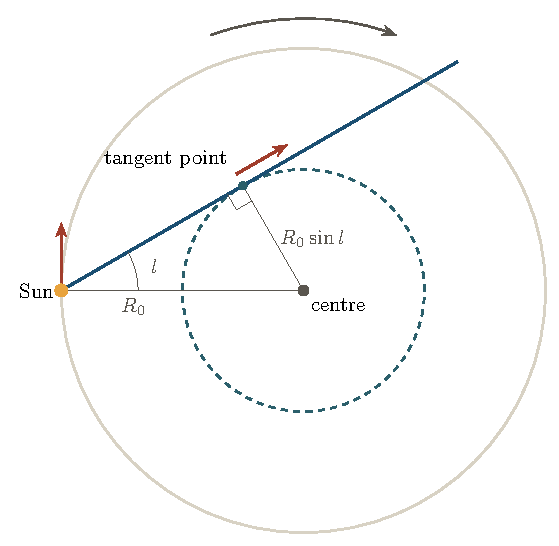
\includegraphics{fig_ch14_tangent.pdf}
	\caption{The Galactic disk seen from the north Galactic pole, to scale, with $R_0=8.2\,\mathrm{kpc}$ and a line of sight at $l=30^\circ$. The grey circle is the Sun's orbit and the dashed circle has radius $R_0\sin l$. The red arrows are the velocities of circular orbits at the Sun and at the tangent point. The arc at the top shows the sense of rotation.}
	\label{ga:fig:tangent}
\end{figure}

\paragraph{The tangent point.} Along a line of sight with $0<l<90^\circ$, the distance from the centre is smallest where the line touches a circle about the centre, at $r=R_0\sin l$ (Figure~\ref{ga:fig:tangent}). If the angular speed $\omega=v_{\rm circ}/r$ falls outward, as it does for a flat or slowly rising curve, it is largest there, and so is $v_r$. Setting $r=R_0\sin l$ in Eq.~\eqref{ga:eq:vr_los},
\begin{align}
	v_{r,\max}
	&= \left(\frac{v_{\rm circ}(R_0\sin l)}{R_0\sin l}-\frac{v_0}{R_0}\right)R_0\sin l
	= v_{\rm circ}(R_0\sin l)-v_0\sin l,
\end{align}
so
\begin{equation}
	\boxed{v_{\rm circ}(R_0\sin l)=v_{r,\max}+v_0\sin l.}
	\label{ga:eq:tangent}
\end{equation}
The highest velocity in the $21\,\mathrm{cm}$ line at each longitude gives the rotation speed at one radius, with no distance needed except $R_0$. Sweeping $l$ from $0$ to $90^\circ$ maps $v_{\rm circ}$ from the centre out to $R_0$. Outside the Sun's circle the method fails, because $r$ grows all along the line. There the distances of the gas or of stars must be found separately, from Cepheids or from \emph{Gaia} parallaxes.

\paragraph{Flat rotation curves.} In our Galaxy, $v_{\rm circ}$ stays between about $200$ and $240\,\mathrm{km\,s^{-1}}$ from $5\,\mathrm{kpc}$ out to $25\,\mathrm{kpc}$. For another spiral seen at an angle, the Doppler shift across its disk gives the curve directly. The light of a disk falls off exponentially with radius, over a few kiloparsecs, so a few such lengths out nearly all the light is inside. If the light traced the mass, $m(r)$ would stop growing there, and $v_{\rm circ}$ would fall as $r^{-1/2}$, like the speeds of the planets. It does not. In the $21\,\mathrm{cm}$ line, whose gas reaches much further than the stars, the rotation curves of most spirals stay flat as far out as they can be followed, often several times the radius of the visible disk. By Eq.~\eqref{ga:eq:vcirc} the mass keeps growing as $r$ there, and by Eq.~\eqref{ga:eq:rho_flat} the unseen matter has $\rho\propto r^{-2}$.

\paragraph{A model galaxy.} Masses add, so the squares of the speeds add,
\begin{equation}
	v_{\rm circ}^2=\frac{G\big(m_{\rm stars}+m_{\rm halo}\big)}{r}=v_{\rm stars}^2+v_{\rm halo}^2 .
\end{equation}
For the halo take a density that is level in a core of radius $r_c$ and falls as $r^{-2}$ outside, $\rho=\rho_c/(1+r^2/r_c^2)$, with $\rho_c$ the central density. Its mass inside $r$ is
\begin{align}
	m_{\rm halo}(r)
	&\eqby{1} \int_0^r\frac{4\pi r'^2\rho_c}{1+r'^2/r_c^2}\,dr' \nonumber\\
	&\eqby{2} 4\pi\rho_cr_c^2\int_0^r\left(1-\frac{1}{1+r'^2/r_c^2}\right)dr' \nonumber\\
	&\eqby{3} 4\pi\rho_cr_c^2\left(r-r_c\arctan\frac{r}{r_c}\right).
\end{align}
\begin{explain}
	\item Eq.~\eqref{pr:eq:mass_inside}.
	\item $r'^2/(1+r'^2/r_c^2)=r_c^2\big[1-1/(1+r'^2/r_c^2)\big]$.
	\item $\int_0^r dr'/(1+r'^2/r_c^2)=r_c\arctan(r/r_c)$.
\end{explain}
By Eq.~\eqref{ga:eq:vcirc},
\begin{equation}
	\boxed{v_{\rm halo}^2=4\pi G\rho_cr_c^2\left[1-\frac{r_c}{r}\arctan\frac{r}{r_c}\right].}
	\label{ga:eq:halo_v}
\end{equation}
Near the centre, $\arctan x\approx x-x^3/3$ gives $v_{\rm halo}^2\approx\tfrac43\pi G\rho_c r^2$, the uniform sphere with $v\propto r$. Far out, $\arctan\to\pi/2$ and $v_{\rm halo}^2\to4\pi G\rho_cr_c^2$, the flat curve. Figure~\ref{ga:fig:rotation} adds this halo to a round model of the stars. The stars set the curve inside a few kiloparsecs and the halo outside, and between them the total is nearly level. The halo's mass grows as $r$ without end, so a real halo must be cut off somewhere. The motions of satellite galaxies show that the Milky Way's halo reaches $200$ to $300\,\mathrm{kpc}$ and holds about $10^{12}\,M_\odot$.

\begin{figure}[htbp]
	\centering
	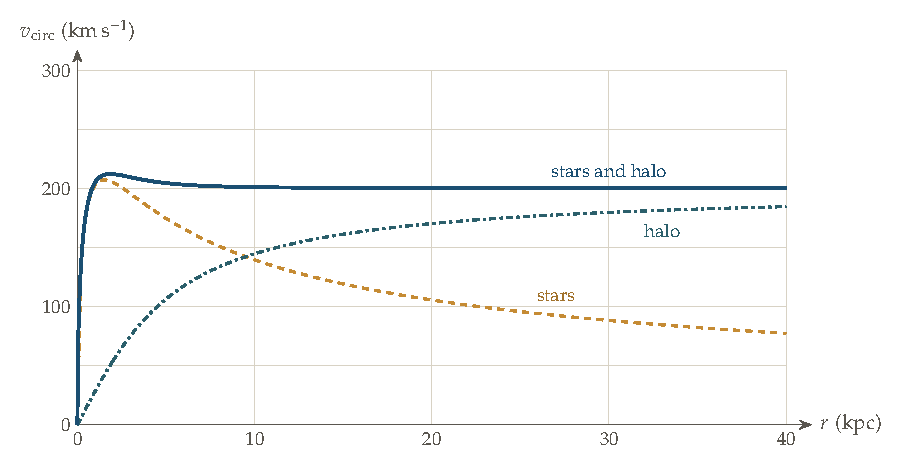
\includegraphics{fig_ch14_rotation.pdf}
	\caption{The circular speed of a model galaxy against radius. Dashed, stars with enclosed mass $6\times10^{10}\,M_\odot\,r^2/(r+1.5\,\mathrm{kpc})^2$. Dash-dotted, the halo of Eq.~\eqref{ga:eq:halo_v} with $r_c=4\,\mathrm{kpc}$ and $4\pi G\rho_cr_c^2=(200\,\mathrm{km\,s^{-1}})^2$. Solid, both together.}
	\label{ga:fig:rotation}
\end{figure}

\paragraph{The mass-to-light ratio.} A galaxy's mass divided by its luminosity, in units of $M_\odot/L_\odot$, is its \textbf{mass-to-light ratio} $M/L$. The Sun has $M/L=1$. A population of old stars has a few, because the mass is mostly in faint low-mass stars and the light comes from the few bright ones. With $L\propto M^{3.5}$ near the Sun (Section~\ref{st:sec:scaling}), a star of $0.5\,M_\odot$ alone has $M/L=0.5^{-2.5}=5.7$. Inside the visible disk of a spiral, the mass from the rotation curve gives $M/L$ of a few, like its stars. Out to the last point of a flat curve it gives ten to several tens, and for clusters of galaxies about three hundred (Section~\ref{ga:sec:weighing}). The ratio grows with the radius inside which the mass is measured, because the unseen matter takes over further out. For the Milky Way, a curve flat at $230\,\mathrm{km\,s^{-1}}$ out to $50\,\mathrm{kpc}$ would put $6\times10^{11}\,M_\odot$ inside that radius, against $6\times10^{10}\,M_\odot$ in stars and gas.

\paragraph{What the unseen mass is not.} It is not cold gas, since the $21\,\mathrm{cm}$ line counts the neutral hydrogen atom by atom (Eq.~\eqref{is:eq:21cm_populations}), and hot gas would shine in X-rays. It is not mostly faint stars or dark compact bodies. Such bodies, crossing in front of stars of the Large Magellanic Cloud, would now and then brighten them by bending their light (Section~\ref{ga:sec:weighing}), and surveys in the 1990s found far too few such events for bodies between about $10^{-7}$ and $10\,M_\odot$ to make up the halo. The amount of ordinary matter of every kind is fixed by the helium and deuterium made in the first minutes of the universe (Chapter~\ref{ch:universe}), and it falls well short of the mass that galaxies need. The halo is mostly a kind of matter that neither sends out nor absorbs light, and it is felt only through its gravity.

% ==============================================================================
\section{Stars as a Gas That Rarely Collides}
\label{ga:sec:relaxation}

The atoms of a gas collide often, and that is what gives them a Maxwell distribution of speeds (P3) and lets a gas be treated as a fluid. The disk of Section~\ref{ga:sec:galaxy} was already treated as a gas of stars.

Stars almost never touch. Near the Sun they are about a parsec apart and a hundred million times smaller than that. A star could cross the Galaxy many times over without hitting another one. If stars never collide, it is not clear that a gas of stars ever forgets how it started, or settles into any kind of equilibrium at all.

Think of a ship crossing the ocean with its rudder tied. Each wave pushes it a little to one side or the other, in no fixed pattern. One wave does nothing worth noticing. But the pushes do not cancel exactly. After many waves the sideways drift has built up, and it grows as the square root of the number of waves. Wait long enough and the ship is heading somewhere else altogether.

A star crossing a galaxy is the ship. Every star it passes tugs it a little, from far away, in a random direction. The tugs add as a random walk in velocity (P5), so the sum of their squares grows steadily. When that sum reaches the square of the star's own speed, the star has forgotten its original orbit. The time this takes is the \textbf{relaxation time}, and comparing it with the age of the system decides what kind of system it is (P6).

The ship in numbers. If each wave pushes it sideways by $1\,\mathrm{cm\,s^{-1}}$ and it sails at $5\,\mathrm{m\,s^{-1}}$, the drift equals the forward speed after $(500)^2=250\,000$ waves. A galaxy of $10^{11}$ stars needs $5\times10^8$ crossings to relax (below), each taking some $5\times10^7$ years. That is $2\times10^{16}$ years, a million times its age. A globular cluster of $10^5$ stars needs only about a thousand crossings of under a million years each, so it relaxes many times over in its life.

The picture is Figure~\ref{ga:fig:encounter}. A star passes a field star on a nearly straight line and gets a small sideways kick toward it. The pulls before and after closest approach have the same sideways part and opposite forward parts.

The same walk in velocity is Brownian motion, and with charges in place of masses it is the way electrons scatter off ions in a plasma (Chapter~\ref{ch:fastparticles}). Here it combines Gauss's law for one kick (P2), the random walk for many (P5) and a comparison of two times (P6). It gives the kick of one passing star, the relaxation time, and what relaxes and what does not.

\begin{figure}[htbp]
	\centering
	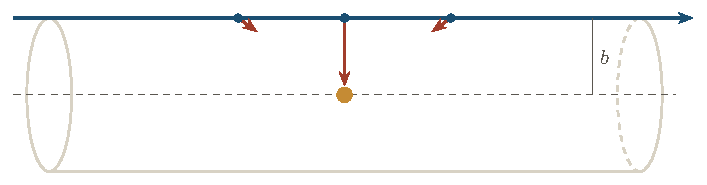
\includegraphics{fig_ch14_encounter.pdf}
	\caption{A star moving left to right along a straight path (blue) passes a field star (dot on the dashed axis) at impact parameter $b$. Red arrows are the pull of the field star at three points of the path. The grey cylinder of radius $b$ about the dashed axis contains the path.}
	\label{ga:fig:encounter}
\end{figure}

\paragraph{One passing star.} Let a star move at speed $v$ past a field star of mass $m_\star$, along a straight line that misses it by the \textbf{impact parameter} $b$. We treat the path as straight and the field star as fixed. Both hold while the kick is small compared with $v$. Put the closest approach at $t=0$, so the star is at distance $\sqrt{b^2+v^2t^2}$. The part of the pull along the path changes sign at $t=0$ and adds nothing. The part across it, toward the line of closest approach, gives the kick,
\begin{align}
	\Delta v
	&\eqby{1} \int_{-\infty}^{\infty}\frac{Gm_\star}{b^2+v^2t^2}\,\frac{b}{\sqrt{b^2+v^2t^2}}\,dt \nonumber\\
	&\eqby{2} \int_{-\pi/2}^{\pi/2}\frac{Gm_\star\,b}{b^3\sec^3\psi}\,\frac bv\sec^2\psi\,d\psi \nonumber\\
	&= \frac{Gm_\star}{bv}\int_{-\pi/2}^{\pi/2}\cos\psi\,d\psi
	= \frac{2Gm_\star}{bv}.
\end{align}
\begin{explain}
	\item The change of velocity is the time integral of the acceleration (P1). The pull is $Gm_\star$ over the distance squared, and the fraction of it across the path is $b$ over the distance.
	\item Substitute $vt=b\tan\psi$, so $dt=(b/v)\sec^2\psi\,d\psi$ and $b^2+v^2t^2=b^2\sec^2\psi$.
\end{explain}
\begin{equation}
	\boxed{\Delta v=\frac{2Gm_\star}{b\,v}.}
	\label{ga:eq:kick}
\end{equation}
The kick is the pull at closest approach, $Gm_\star/b^2$, times about twice the time spent near it, $b/v$. A closer or slower passage gives a larger kick.

\paragraph{The same kick from Gauss's law.} Draw a cylinder of radius $b$ whose axis passes through the field star, parallel to the path (Figure~\ref{ga:fig:encounter}). The path lies on its surface. Let the cylinder be very long, so its ends carry no flux. With $\phi$ the angle round the axis, $x$ the length along it and $g_r$ the part of the pull pointing away from the axis,
\begin{align}
	-4\pi Gm_\star
	&\eqby{1} \oint\vec g\cdot d\vec A
	\eqby{2} \int_0^{2\pi}b\,d\phi\int_{-\infty}^{\infty}g_r\,dx
	\eqby{3} 2\pi b\int_{-\infty}^{\infty}g_r\,dx .
\end{align}
\begin{explain}
	\item Gauss's law \eqref{pr:eq:gauss_gravity}, with $m_\star$ inside (P2).
	\item The area element on the side is $b\,d\phi\,dx$, and only the part of $\vec g$ across the side counts.
	\item Every line on the cylinder parallel to the axis is the same as every other, by symmetry about the axis.
\end{explain}
So $\int g_r\,dx=-2Gm_\star/b$ along the path, and with $dx=v\,dt$ the kick toward the axis is $2Gm_\star/(bv)$, Eq.~\eqref{ga:eq:kick} again. No integral had to be done. The kick depends on the mass of the field star and on $b$, exactly as the field of a line of charge depends on its charge and the distance.

The straight path holds while $\Delta v\ll v$, which is $b\gg2Gm_\star/v^2$. For a star of one solar mass passed at $200\,\mathrm{km\,s^{-1}}$ that is $0.044\,\mathrm{AU}$. Almost every encounter in a galaxy is far wider than this.

\paragraph{Many passing stars.} Take a system of $N$ stars of mass $m_\star$ within a radius $R$, through which a star crosses at a typical speed $v$ in the \textbf{crossing time} $t_{\rm cross}=R/v$. In one crossing it passes through the system's disk on the sky, of area $\pi R^2$ holding $N$ stars. The number of field stars it passes with impact parameters between $b$ and $b+db$ is $(N/\pi R^2)\,2\pi b\,db=2Nb\,db/R^2$. Each kick points across the path in a random direction, so the kicks add as the steps of a random walk. Their squares add, and the cross terms average to zero, as in Eq.~\eqref{pr:eq:sqrtN} (P5). In one crossing,
\begin{align}
	\sum|\Delta\vec v|^2
	&\eqby{1} \int_{b_{\min}}^{R}\left(\frac{2Gm_\star}{bv}\right)^2\frac{2Nb\,db}{R^2} \nonumber\\
	&\eqby{2} 8N\left(\frac{Gm_\star}{Rv}\right)^2\int_{b_{\min}}^{R}\frac{db}{b}
	= 8N\left(\frac{Gm_\star}{Rv}\right)^2\ln\frac{R}{b_{\min}} .
	\label{ga:eq:kicks_sum}
\end{align}
\begin{explain}
	\item The square of Eq.~\eqref{ga:eq:kick}, times the number of passages at each $b$. No star lies further away than about $R$. Below $b_{\min}=2Gm_\star/v^2$ a single kick is as large as $v$ and the straight path fails.
	\item Collect the constants.
\end{explain}
The integral is a logarithm, so each factor of ten in $b$ adds the same amount. The many distant passages together matter more than the rare close ones, and close encounters, the only ones that a contact collision picture would count, add less than one factor of ten out of many.

\paragraph{The relaxation time.} To put Eq.~\eqref{ga:eq:kicks_sum} in terms of $N$ alone, we use the virial theorem (Eq.~\eqref{sg:eq:virial_dynamic} with $\ddot I=0$, $2K=|U|$) in order of magnitude, $v^2\approx GNm_\star/R$. Then $Gm_\star/R=v^2/N$ and $b_{\min}=2R/N$, and the relative size of the summed kicks in one crossing is
\begin{align}
	\frac{\sum|\Delta\vec v|^2}{v^2}
	&\eqby{1} \frac{8N}{v^2}\left(\frac vN\right)^2\ln\frac N2 \nonumber\\
	&\eqby{2} \frac{8\ln N}{N}.
\end{align}
\begin{explain}
	\item Eq.~\eqref{ga:eq:kicks_sum} with $Gm_\star/(Rv)=v/N$ and $R/b_{\min}=N/2$.
	\item For large $N$, $\ln(N/2)$ and $\ln N$ differ by less than the cut-offs at $R$ and $b_{\min}$ are known.
\end{explain}
The star's speed has been changed by an amount comparable to itself after $N/(8\ln N)$ crossings,
\begin{equation}
	\boxed{t_{\rm relax}=\frac{N}{8\ln N}\,t_{\rm cross},\qquad t_{\rm cross}=\frac Rv .}
	\label{ga:eq:trelax}
\end{equation}
Only the number of stars and the crossing time enter. For a given crossing time, a system of fewer, heavier stars relaxes faster, because each kick is larger.

\paragraph{What relaxes.} Table~\ref{ga:tab:relax} puts in the numbers, with $v$ from $v^2=GM/R$.
\begin{table}[htbp]
	\centering
	\begin{tabular}{@{}l c c c c c c c@{}}
		\toprule
		\textbf{System} & $M$ ($M_\odot$) & $N$ & $R$ & $v$ ($\mathrm{km\,s^{-1}}$) & $t_{\rm cross}$ (yr) & $t_{\rm relax}$ (yr) & age (yr) \\
		\midrule
		Open cluster & $500$ & $10^3$ & $2\,\mathrm{pc}$ & $1.0$ & $1.9\times10^6$ & $3\times10^7$ & $10^8$ \\
		Globular cluster & $5\times10^4$ & $10^5$ & $5\,\mathrm{pc}$ & $6.6$ & $7.5\times10^5$ & $8\times10^8$ & $1.2\times10^{10}$ \\
		Galaxy & $10^{11}$ & $10^{11}$ & $10\,\mathrm{kpc}$ & $207$ & $4.7\times10^7$ & $2\times10^{16}$ & $10^{10}$ \\
		\bottomrule
	\end{tabular}
	\caption{Crossing and relaxation times, Eq.~\eqref{ga:eq:trelax}, for three kinds of star system.}
	\label{ga:tab:relax}
\end{table}
The ratio $t_{\rm relax}/\text{age}$ sorts them (P6). In a galaxy it is a million. Its stars have never traded energy with each other. Each moves in the smooth pull of the whole galaxy as if the other stars were spread out into a fluid, and a galaxy is \textbf{collisionless}. In a globular cluster the ratio is about a tenth, so the cluster has relaxed many times.

\paragraph{Galaxies remember.} A collisionless galaxy keeps the orbits its stars were born on. Near the Sun the spread of stellar velocities is larger toward the Galactic centre than up out of the plane. A relaxed gas would have made it the same in every direction, as collisions do for the pressure of a gas. The vertical balance of Section~\ref{ga:sec:galaxy} needed only $\Pi_{zz}$, so it still holds. The disk does heat slowly, and old stars move faster than young ones, but the heating comes from the much larger kicks of giant molecular clouds and spiral arms, not from single stars. The shapes of galaxies, too, are set when they form and kept since (Section~\ref{ga:sec:normal}).

\paragraph{Globular clusters relax, and lose stars.} In a cluster that relaxes, kicks drive the speeds toward a Maxwell distribution (P3 and P4). Its fastest stars then have more than the escape speed and leave. To see how many, compare the escape speed with the mean square speed. Let $\Phi$ be the gravitational potential, so that a star at rest at infinity has $\tfrac12v_{\rm esc}^2+\Phi=0$, and $U=\tfrac12\int\Phi\,dm$, since a sum over the potential of every mass element counts each pair twice. Averaging over the mass,
\begin{align}
	\avg{v_{\rm esc}^2}
	&\eqby{1} -\frac2M\int\Phi\,dm
	\eqby{2} -\frac{4U}{M}
	\eqby{3} \frac{8K}{M}
	\eqby{4} 4\avg{v^2}.
	\label{ga:eq:vesc}
\end{align}
\begin{explain}
	\item $v_{\rm esc}^2=-2\Phi$ (P1 for energy), averaged over the mass $M$.
	\item $\int\Phi\,dm=2U$.
	\item The virial theorem, $2K+U=0$, Eq.~\eqref{sg:eq:virial_dynamic} averaged in time.
	\item $K=\tfrac12M\avg{v^2}$.
\end{explain}
A star escapes once its speed exceeds about twice the root-mean-square speed. In a Maxwell distribution with $\avg{v^2}=3\sigma^2$, where $\sigma$ is the spread of one velocity component, the fraction of stars faster than $2\sqrt3\,\sigma$ is
\[
\int_{2\sqrt3\,\sigma}^{\infty}\frac{4\pi v^2}{(2\pi\sigma^2)^{3/2}}\,e^{-v^2/2\sigma^2}\,dv
=\operatorname{erfc}\sqrt6+2\sqrt{\frac6\pi}\,e^{-6}=0.0074 ,
\]
where the integral was done by parts. Relaxation refills this tail once in every relaxation time, so the cluster loses $0.74$ per cent of its stars per $t_{\rm relax}$ and would evaporate in about $135\,t_{\rm relax}$, some $10^{11}$ years for the cluster of Table~\ref{ga:tab:relax}. The tidal pull of the Galaxy strips the outer stars and shortens this. Relaxation also shares energy between stars of different mass. Heavy stars lose speed, sink toward the centre, and leave the light ones in the outskirts.

\paragraph{Core collapse.} The dense core of a globular cluster is a self-gravitating system, with the negative heat capacity of Section~\ref{sg:sec:negheat}. Its stars move faster than those of the outer parts, so relaxation carries energy outward, as heat flows from a hot body to a cold one. The core loses energy, and with $C<0$ it gets hotter and contracts. A hotter core passes energy to the outer parts even faster, and the process runs away. This is the \textbf{gravothermal catastrophe}. The core shrinks toward a very small, very dense centre. It is stopped by close pairs of stars that form there. When a third star passes close to a pair, the pair binds tighter and the third star leaves faster, so the pair hands energy to the core and heats it. About a fifth of the globular clusters of the Milky Way have the sharply peaked centres that mark a collapsed core. A galaxy, whose relaxation time is a million times its age, never gets there.

% ==============================================================================
\section{Weighing Galaxies and Clusters}
\label{ga:sec:weighing}

A disk is weighed by its rotation, Eq.~\eqref{ga:eq:vcirc}. The virial theorem of Section~\ref{sg:sec:virial} ties the kinetic and gravitational energies of any bound system in a steady state.

Elliptical galaxies and clusters of galaxies do not rotate in an orderly way. Their members move in every direction. We see only the speed along the line of sight and the position on the sky, not the full motion or the depth.

Think of a salad bowl full of marbles, shaken and watched from above. The bowl itself cannot be seen. But marbles that move fast stay inside only if the bowl is deep, and from how fast they move and how far they spread one can judge its depth.

The galaxies of a cluster are the marbles, and the cluster's gravity is the bowl. In 1933 Zwicky measured the line-of-sight speeds of galaxies in the Coma cluster, spread by about $1000\,\mathrm{km\,s^{-1}}$ over a few megaparsecs, and found that the bowl must hold hundreds of times the mass of the stars in it. The virial theorem turns random speeds and sizes into a mass.

A uniform sphere in numbers. With the virial theorem $2K=|U|$, $K=\tfrac12M\cdot3\sigma^2$ for a line-of-sight spread $\sigma$, and $|U|=\tfrac35GM^2/R$ (Eq.~\eqref{sg:eq:U_uniform}), the mass is $M=5\sigma^2R/G$. For $\sigma=1000\,\mathrm{km\,s^{-1}}$ and $R=1.5\,\mathrm{Mpc}$ it is $1.7\times10^{15}\,M_\odot$.

The picture is a cluster on the sky, a swarm of dots, each with one arrow along the line of sight.

The same reasoning gave the temperature of a star from its gravity (Eq.~\eqref{sg:eq:virial_T}). For the hot gas of a cluster it becomes hydrostatic equilibrium again (P1 and P2), and the bending of light by mass, from general relativity, weighs a cluster with no reference to motion at all. It gives the mass from line-of-sight speeds and positions on the sky, the mass from the hot gas, and the mass from the bending of light.

\paragraph{From three dimensions to what is seen.} Take $N$ galaxies of equal mass $m_\star$, total mass $M=Nm_\star$, in a steady state. Their kinetic energy is $K=\tfrac12M\avg{v^2}$. We measure only the line-of-sight component, with mean square $\sigma^2$ after the mean motion of the cluster is removed. If the motions favour no direction,
\begin{align}
	\avg{v^2}
	&= \avg{v_x^2}+\avg{v_y^2}+\avg{v_z^2}
	\eqby{1} 3\sigma^2 ,
\end{align}
\begin{explain}
	\item With no favoured direction, each component has the same mean square as the one along the line of sight.
\end{explain}
The gravitational energy is a sum over pairs, $U=-Gm_\star^2\sum_{\rm pairs}1/r$, with $\tfrac12N(N-1)$ pairs. We see each separation $r$ projected on the sky, $r_\perp=r\sin\theta$, where $\theta$ is the angle between the separation and the line of sight. The direction of a pair has nothing to do with its separation, so the two can be averaged one at a time over all pairs,
\begin{align}
	\avg{\frac1{r_\perp}}
	&\eqby{1} \avg{\frac1r}\avg{\frac{1}{\sin\theta}}
	\eqby{2} \avg{\frac1r}\frac{1}{4\pi}\int_0^{2\pi}\!\!\int_0^\pi\frac{1}{\sin\theta}\,\sin\theta\,d\theta\,d\phi
	\eqby{3} \frac\pi2\avg{\frac1r} .
\end{align}
\begin{explain}
	\item $r$ and $\theta$ are independent.
	\item All directions equally likely, with the solid angle $\sin\theta\,d\theta\,d\phi$ over $4\pi$.
	\item The integrand is $1$, so the integral is $2\pi\cdot\pi$.
\end{explain}
\paragraph{The virial mass.} Setting $2K=|U|$,
\begin{align}
	M\cdot3\sigma^2
	&\eqby{1} Gm_\star^2\,\frac{N(N-1)}{2}\avg{\frac1r} \nonumber\\
	&\eqby{2} Gm_\star^2\,\frac{N(N-1)}{2}\,\frac2\pi\avg{\frac{1}{r_\perp}}
	= \frac{GM^2}{\pi}\left(1-\frac1N\right)\avg{\frac1{r_\perp}} .
\end{align}
\begin{explain}
	\item The virial theorem, Eq.~\eqref{sg:eq:virial_dynamic} averaged in time, with $K$ and $U$ from above.
	\item The projection factor $\pi/2$.
\end{explain}
For $N\gg1$,
\begin{equation}
	\boxed{M=\frac{3\pi\,\sigma^2}{G\avg{1/r_\perp}}.}
	\label{ga:eq:Mvir}
\end{equation}
Only line-of-sight speeds and positions on the sky enter, with the distance to the cluster needed to turn angles into $r_\perp$. The result assumes a steady state, motions with no favoured direction, and galaxies that are spread like the mass. It does not depend on what the mass is made of. As a check, a uniform sphere has $\avg{1/r}=|U|/(Gm_\star^2N^2/2)=6/(5R)$ by Eq.~\eqref{sg:eq:U_uniform}, so $\avg{1/r_\perp}=3\pi/(5R)$, and Eq.~\eqref{ga:eq:Mvir} gives $M=5\sigma^2R/G$, the value found above.

For a cluster with $\sigma=1000\,\mathrm{km\,s^{-1}}$ and $1/\avg{1/r_\perp}=1\,\mathrm{Mpc}$, Eq.~\eqref{ga:eq:Mvir} gives $2.2\times10^{15}\,M_\odot$. Coma has a mass of about $10^{15}\,M_\odot$ and a mass-to-light ratio of about $300$. Its galaxies shine with a few tenths of a per cent of the light that this mass would give if it were all stars like the Sun.

\paragraph{The hot gas.} The same well holds the hot gas between the galaxies. Its particles share the energy per unit mass of the galaxies, so $k_BT=\mu m_{\rm H}\sigma^2$, about $7\times10^7\,\mathrm K$ for $\sigma=1000\,\mathrm{km\,s^{-1}}$ (Problem~\ref{sg:prob:cluster}). Gas this hot shines in X-rays by bremsstrahlung (Eq.~\eqref{fp:eq:brems_total} and Problem~\ref{fp:prob:cluster}), and X-ray telescopes measure its temperature and density at each radius. Hydrostatic equilibrium then gives the mass. With $P=\rho k_BT/(\mu m_{\rm H})$,
\begin{align}
	-\frac{G\,m(r)\,\rho}{r^2}
	&\eqby{1} \dv{P}{r}
	\eqby{2} \frac{k_B}{\mu m_{\rm H}}\left(T\dv{\rho}{r}+\rho\dv{T}{r}\right) \nonumber\\
	&\eqby{3} \frac{\rho\,k_BT}{\mu m_{\rm H}\,r}\left(\dv{\ln\rho}{\ln r}+\dv{\ln T}{\ln r}\right).
\end{align}
\begin{explain}
	\item Hydrostatic equilibrium, Eq.~\eqref{sg:eq:hse}.
	\item The ideal gas, differentiated.
	\item $\dv*{\rho}{r}=(\rho/r)\,\dv*{\ln\rho}{\ln r}$, and the same for $T$.
\end{explain}
\begin{equation}
	\boxed{m(r)=-\frac{k_BT\,r}{G\mu m_{\rm H}}\left(\dv{\ln\rho}{\ln r}+\dv{\ln T}{\ln r}\right).}
	\label{ga:eq:mX}
\end{equation}
Only the temperature and the slopes of the profiles enter, not the amount of gas. For gas at one temperature with $\rho\propto r^{-2}$, the bracket is $-2$ and $m=2k_BTr/(G\mu m_{\rm H})$. With $k_BT=\mu m_{\rm H}\sigma^2$ this is $m=2\sigma^2r/G$, the isothermal sphere of Section~\ref{st:sec:polytropes} with $v_{\rm circ}^2=2\sigma^2$, which is a second route to the same mass. Inside $1\,\mathrm{Mpc}$ it is $4.6\times10^{14}\,M_\odot$. The gas itself holds several times the mass of the stars, yet stars and gas together are only about a sixth of the total.

\paragraph{The bending of light.} General relativity bends a ray that passes a mass $M$ at impact parameter $b$ through the angle $4GM/(bc^2)$, twice the Newtonian value. For a lens that is not a point, $M$ is the mass inside the circle of radius $b$ on the sky, if the lens is round. Put a source directly behind a lens, at distance $D_S$ from us, with the lens at $D_L$ and $D_{LS}$ between the two (Figure~\ref{ga:fig:lens}). A ray we see at a small angle $\theta$ from the lens passes it at $b=\theta D_L$. Without bending it would reach the source's distance at the height $\theta D_S$. Bent back toward the axis, it reaches that distance at the height $\theta D_S-4GMD_{LS}/(bc^2)$, and it comes from the source only if this is zero,
\begin{align}
	\theta D_S
	&\eqby{1} \frac{4GM}{bc^2}\,D_{LS}
	\eqby{2} \frac{4GM}{\theta D_Lc^2}\,D_{LS}
	\quad\implies\quad
	\theta^2=\frac{4GM}{c^2}\,\frac{D_{LS}}{D_LD_S} .
\end{align}
\begin{explain}
	\item The height of the bent ray at the source, set to zero, with small angles.
	\item $b=\theta D_L$.
\end{explain}
\begin{equation}
	\boxed{\theta_E=\sqrt{\frac{4GM}{c^2}\,\frac{D_{LS}}{D_LD_S}}}
	\label{ga:eq:einstein}
\end{equation}
By symmetry the source appears as a ring of this angular radius, the \textbf{Einstein ring}. A source a little off the axis appears as two images or as arcs near the ring. Only the mass inside the ring enters, not how it moves or what state it is in. For $10^{14}\,M_\odot$ with $D_L=1\,\mathrm{Gpc}$ and $D_S=2\,\mathrm{Gpc}$, $\theta_E=20''$, and rich clusters do show arcs of about this size. A galaxy of $10^{11}\,M_\odot$ gives $0.6''$. At such distances the $D$s are the distances of Chapter~\ref{ch:universe} that relate size to angle, for which $D_L+D_{LS}\neq D_S$. The formula keeps its form. Masses from lensing, from the galaxies' speeds and from the hot gas agree within a few tens of per cent. In the colliding pair of clusters called the Bullet Cluster, the lensing mass sits with the galaxies, while most of the ordinary matter, the gas, has been slowed and left between them.

\begin{figure}[htbp]
	\centering
	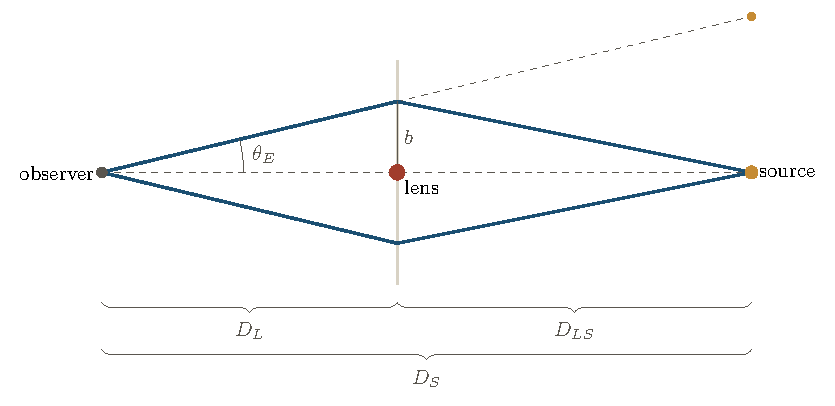
\includegraphics{fig_ch14_lens.pdf}
	\caption{A source directly behind a lens. Two rays from the source are bent at the lens plane and reach the observer at the angle $\theta_E$ from the lens. The dashed line continues the direction in which the observer sees the upper image. Angles are exaggerated.}
	\label{ga:fig:lens}
\end{figure}

% ==============================================================================
\section{Normal Galaxies}
\label{ga:sec:normal}

A galaxy can be weighed by its rotation, Eq.~\eqref{ga:eq:vcirc}, or by the random speeds of its stars, Eq.~\eqref{ga:eq:Mvir}.

Weighing gives a mass. It does not say how bright a galaxy really is, or how far away, and galaxies come in very different shapes. What is wanted is a link between the motions, which are easy to measure, and the true luminosity.

Think of apples from one orchard. They are all about equally dense. Measure the width of an apple and you know its weight without a scale, because the weight grows as the cube of the width. One fixed property turns one measured quantity into another, through a power law.

Spiral disks are like the apples. They have nearly the same surface brightness, and their stars nearly the same mass-to-light ratio. With $v_{\rm circ}^2=Gm/R$ these two fixed ratios make the luminosity grow as the fourth power of the rotation speed. The width of the $21\,\mathrm{cm}$ line then gives the luminosity, and the luminosity with the observed flux gives the distance. A power law follows from the virial theorem and two fixed ratios.

The apples in numbers. An apple twice as wide is $2^3=8$ times heavier. A spiral that rotates twice as fast is $2^4=16$ times brighter, $2.5\log_{10}16=3.0$ magnitudes.

The picture is a plot of luminosity against rotation speed on logarithmic axes, where spirals lie close to a straight line of slope four.

The same kind of scaling gave the mass–luminosity relation of stars (Section~\ref{st:sec:scaling}, P6). With random speeds in place of rotation it works for elliptical galaxies. It gives the main kinds of galaxies, the two scaling laws, and how they measure distances.

\paragraph{The Hubble sequence.} Hubble sorted galaxies by their look into a sequence. \textbf{Ellipticals} are smooth and featureless, labelled E0 to E7 by how flattened they appear. \textbf{Lenticulars}, S0, have a disk but no spiral arms. \textbf{Spirals} run from Sa, with a large bulge and tightly wound arms, to Sd, with a small bulge and open arms, and those with a bar form a parallel sequence SBa to SBd. \textbf{Irregulars} fit nowhere. Along the sequence from ellipticals to late spirals, the fraction of gas and of young blue stars grows, and the support against gravity changes. Ellipticals are held up by random motions of $100$ to $300\,\mathrm{km\,s^{-1}}$ and rotate little. Their stars are old and red, and they have little cold gas. Disks are held up by rotation at $100$ to $300\,\mathrm{km\,s^{-1}}$, with random motions of only a few tens. A collisionless galaxy keeps the motions it formed with (Section~\ref{ga:sec:relaxation}), so its shape records its history. Mergers of disk galaxies, which mix the orbits violently, can make ellipticals.

\paragraph{Tully–Fisher from the virial theorem.} Let a disk of radius $R$ have mass $M$ inside $R$ and luminosity $L$. Its rotation speed is $v^2=GM/R$ by Eq.~\eqref{ga:eq:vcirc}. Suppose $M/L$ and the surface brightness, measured by $L/R^2$, are the same for all such disks. To get $L$ in terms of $v$ alone, we write $M$ and $R$ through these two ratios,
\begin{align}
	L
	&\eqby{1} \left(\frac LM\right)M
	\eqby{2} \left(\frac LM\right)\frac{v^2R}{G}
	\eqby{3} \left(\frac LM\right)\frac{v^2}{G}\left(\frac{R^2}{L}\right)^{1/2}L^{1/2} .
\end{align}
\begin{explain}
	\item The mass-to-light ratio.
	\item Eq.~\eqref{ga:eq:vcirc} at the edge of the disk.
	\item $R=(R^2/L)^{1/2}L^{1/2}$.
\end{explain}
Dividing by $L^{1/2}$ and squaring,
\begin{equation}
	\boxed{L=\left(\frac LM\right)^2\left(\frac{R^2}{L}\right)\frac{v^4}{G^2}.}
	\label{ga:eq:tf}
\end{equation}
This is the \textbf{Tully–Fisher relation}, $L\propto v^4$. The power four comes from the virial theorem and the fixed surface brightness. The constant in front holds the two ratios that were assumed fixed. The observed relation is close to $L\propto v^4$ in the near infrared, where the light traces the old stars, and it is tight. Disks do have nearly the same central surface brightness, which explains part of it. Yet $v$ is set mostly by the dark halo and $L$ by the stars, and galaxies of low surface brightness lie on the same relation. Why the halo and the stars keep the relation so tight is not explained by the virial theorem. Counting the gas with the stars makes the relation tighter still.

\paragraph{Faber–Jackson.} For an elliptical galaxy, the uniform-sphere form of the virial theorem from Section~\ref{ga:sec:weighing}, $M=5\sigma^2R/G$, takes the place of $M=v^2R/G$. The same three steps with $v^2$ replaced by $5\sigma^2$ give
\begin{equation}
	\boxed{L=25\left(\frac LM\right)^2\left(\frac{R^2}{L}\right)\frac{\sigma^4}{G^2},}
	\label{ga:eq:fj}
\end{equation}
the \textbf{Faber–Jackson relation} $L\propto\sigma^4$. It holds less tightly than Tully–Fisher, because the surface brightness of ellipticals is not fixed. Keeping $L/R^2$ as a third measured quantity turns the line into a plane in the space of $R$, $\sigma$ and surface brightness, the fundamental plane, on which ellipticals lie closely.

\paragraph{Distances.} The $21\,\mathrm{cm}$ line of a whole spiral is broadened by its rotation. The side moving toward us and the side moving away shift the line by $\pm v\sin\iota$, where $\iota$ is the inclination of the disk to the sky ($\iota=90^\circ$ for a disk seen edge on), so the full width is $W=2v\sin\iota$. A thin round disk tilted by $\iota$ looks like an ellipse with axis ratio $\cos\iota$, which gives $\iota$. Then $v$ gives $L$ by Eq.~\eqref{ga:eq:tf}, once the constant has been fixed with galaxies of known distance. In magnitudes, $L\propto v^4$ means that the absolute magnitude changes by $-10\log_{10}$ of the ratio of rotation speeds (Eq.~\eqref{eq:pogson_difference}), and the distance follows from the distance modulus, Eq.~\eqref{eq:distance_modulus} (Problem~\ref{ga:prob:tf}). Tully–Fisher distances reach a few hundred megaparsecs, where the expansion of the universe (Chapter~\ref{ch:universe}) takes over as a measure of distance.

% ==============================================================================
\section{Problem Set: Galaxies and the Motions of Stars}

\subsection{Problem 1: The Sun's Orbit and the Local Dark Matter}
\label{ga:prob:sun}

\textbf{Problem Statement}: The Sun circles the Galactic centre at $v_0=230\,\mathrm{km\,s^{-1}}$ at $R_0=8.2\,\mathrm{kpc}$. (a) How long does one orbit take? (b) How many orbits has the Sun made in its $4.6\times10^9$ years? (c) What mass lies inside the Sun's orbit? (d) If the rotation curve is flat and all the mass is in a round halo, what is the density at the Sun, in $M_\odot\,\mathrm{pc^{-3}}$ and in $\mathrm{GeV}\,c^{-2}\,\mathrm{cm^{-3}}$? (e) How much of this density lies in a slab within $1.1\,\mathrm{kpc}$ of the plane, per unit area? Compare with the $20\,M_\odot\,\mathrm{pc^{-2}}$ by which the weighed disk exceeds the visible stars and gas.

\textbf{Essential Ideas}:
\begin{itemize}
	\item The circular speed weighs the mass inside, $v_{\rm circ}^2=Gm(r)/r$, Eq.~\eqref{ga:eq:vcirc}.
	\item A flat curve has $\rho=v_{\rm circ}^2/(4\pi Gr^2)$, Eq.~\eqref{ga:eq:rho_flat}.
\end{itemize}

\textbf{Detailed Solutions}:
\begin{enumerate}[label=(\alph*)]
	\item \textbf{Period}. $2\pi R_0/v_0=2\pi\times8.2\times3.086\times10^{19}\,\mathrm m/(2.3\times10^5\,\mathrm{m\,s^{-1}})$.
	\[
	\boxed{2.2\times10^8\ \text{years}.}
	\]
	\item \textbf{Number of orbits}. $4.6\times10^9/2.19\times10^8$.
	\[
	\boxed{\text{about }21.}
	\]
	\item \textbf{Mass inside}. $m=v_0^2R_0/G=(2.3\times10^5)^2\times2.53\times10^{20}/6.674\times10^{-11}\,\mathrm{kg}$.
	\[
	\boxed{m(R_0)=1.0\times10^{11}\,M_\odot.}
	\]
	\item \textbf{Local density}. $\rho=v_0^2/(4\pi GR_0^2)=9.9\times10^{-22}\,\mathrm{kg\,m^{-3}}$. Multiplying by $c^2$ and dividing by $1.602\times10^{-10}\,\mathrm{J\,GeV^{-1}}$ and $10^6\,\mathrm{cm^3\,m^{-3}}$,
	\[
	\boxed{\rho=0.015\,M_\odot\,\mathrm{pc^{-3}}=0.55\,\mathrm{GeV}\,c^{-2}\,\mathrm{cm^{-3}}.}
	\]
	This overestimates the halo, since the disk also supplies part of $v_0$. Careful models give about two thirds of it.
	\item \textbf{In the slab}. $0.015\,M_\odot\,\mathrm{pc^{-3}}\times2200\,\mathrm{pc}$.
	\[
	\boxed{\approx30\,M_\odot\,\mathrm{pc^{-2}},}
	\]
	or about $20$ with the smaller halo density of (d). This matches the excess found by weighing the disk. The unseen mass near the Sun is what a round halo puts there, with no extra dark matter in the disk itself.
\end{enumerate}

\subsection{Problem 2: Weighing the Disk}
\label{ga:prob:disk}

\textbf{Problem Statement}: (a) A population of old stars of the thick disk has a vertical velocity spread $\sigma_z=40\,\mathrm{km\,s^{-1}}$, the same at every height, and its number falls with height with the scale $h_z=900\,\mathrm{pc}$. Find the mass per unit area of the disk. (b) Near the plane, take the disk to be a uniform slab of density $\rho_0=0.1\,M_\odot\,\mathrm{pc^{-3}}$. Show that a star inside it oscillates up and down harmonically, and find the period. How often does the Sun cross the plane? (c) The derivation of Eq.~\eqref{ga:eq:disk_height} used a pressure, yet stars do not collide. Why is that allowed?

\textbf{Essential Ideas}:
\begin{itemize}
	\item $h_z=\sigma_z^2/(2\pi G\Sigma)$, Eq.~\eqref{ga:eq:disk_height}.
	\item Gauss's law \eqref{pr:eq:gauss_gravity} for a box inside the slab.
\end{itemize}

\textbf{Detailed Solutions}:
\begin{enumerate}[label=(\alph*)]
	\item \textbf{Mass per area}. $\Sigma=\sigma_z^2/(2\pi Gh_z)=(4\times10^4)^2/(2\pi\times6.674\times10^{-11}\times2.78\times10^{19})\,\mathrm{kg\,m^{-2}}$.
	\[
	\boxed{\Sigma\simeq66\,M_\odot\,\mathrm{pc^{-2}}.}
	\]
	\item \textbf{Vertical oscillation}. A box with faces at $\pm z$ inside the slab holds the mass $2z\rho_0A$, so Gauss's law gives $2g(z)A=4\pi G\rho_0\,2zA$, and $g=4\pi G\rho_0z$ toward the plane. Then $\ddot z=-4\pi G\rho_0\,z$, a harmonic oscillation with angular frequency $\sqrt{4\pi G\rho_0}$. With $\rho_0=6.77\times10^{-21}\,\mathrm{kg\,m^{-3}}$,
	\[
	\boxed{\text{period}=\frac{2\pi}{\sqrt{4\pi G\rho_0}}\simeq84\ \text{million years}.}
	\]
	The Sun crosses the plane twice per period, about every $42$ million years. The period does not depend on how far the star swings, as long as it stays inside the slab.
	\item \textbf{No collisions needed}. The pressure in the momentum equation is the momentum carried across a surface by particles moving through it, Eq.~\eqref{pr:eq:momentum_flux}. Counting that flow needs only the particles' velocities, not collisions. What collisions would add is the same spread of speeds in every direction. The vertical balance uses only $\Pi_{zz}=\rho\sigma_z^2$, so it holds for stars whatever their spread in other directions.
\end{enumerate}

\subsection{Problem 3: Relaxation and Evaporation of a Globular Cluster}
\label{ga:prob:gc}

\textbf{Problem Statement}: A globular cluster holds $N=2\times10^5$ stars with a total mass of $10^5\,M_\odot$ within $R=5\,\mathrm{pc}$. Estimate (a) the typical speed of its stars, (b) the crossing time, (c) the relaxation time, and (d) the evaporation time. (e) The cluster is $1.2\times10^{10}$ years old. Is it relaxed? Should it still exist?

\textbf{Essential Ideas}:
\begin{itemize}
	\item $v^2\approx GM/R$ from the virial theorem in order of magnitude.
	\item $t_{\rm relax}=N/(8\ln N)\,t_{\rm cross}$, Eq.~\eqref{ga:eq:trelax}.
	\item A relaxed cluster loses $0.74$ per cent of its stars per relaxation time, Eq.~\eqref{ga:eq:vesc} and the Maxwell tail.
\end{itemize}

\textbf{Detailed Solutions}:
\begin{enumerate}[label=(\alph*)]
	\item \textbf{Speed}. $v=\sqrt{GM/R}=\sqrt{6.674\times10^{-11}\times1.989\times10^{35}/1.543\times10^{17}}\,\mathrm{m\,s^{-1}}$.
	\[
	\boxed{v\simeq9.3\,\mathrm{km\,s^{-1}}.}
	\]
	\item \textbf{Crossing time}. $R/v=1.543\times10^{17}/9.28\times10^3\,\mathrm s$.
	\[
	\boxed{t_{\rm cross}\simeq5.3\times10^5\ \text{years}.}
	\]
	\item \textbf{Relaxation time}. $N/(8\ln N)=2\times10^5/(8\times12.2)=2050$.
	\[
	\boxed{t_{\rm relax}\simeq1.1\times10^9\ \text{years}.}
	\]
	\item \textbf{Evaporation time}. $t_{\rm relax}/0.0074$.
	\[
	\boxed{t_{\rm evap}\simeq1.5\times10^{11}\ \text{years}.}
	\]
	\item \textbf{Age}. The cluster is about $11$ relaxation times old, so its stars have shared their energy and its heavy stars have sunk toward the centre. Evaporation alone would take more than ten times its age, so it survives. The Galaxy's tides and the shocks of crossing the disk remove stars faster, and many clusters that were once smaller or looser have already dissolved into the halo.
\end{enumerate}

\subsection{Problem 4: One Cluster, Three Weighings}
\label{ga:prob:cluster3}

\textbf{Problem Statement}: Model a rich cluster as an isothermal sphere, $\rho=\sigma^2/(2\pi Gr^2)$, with line-of-sight spread $\sigma=1000\,\mathrm{km\,s^{-1}}$ for its galaxies and hot gas of $\mu=0.6$ at $k_BT=\mu m_{\rm H}\sigma^2$. (a) Find the mass inside $1\,\mathrm{Mpc}$ from the X-ray gas. (b) Show that it equals $v_{\rm circ}^2r/G$ for this sphere. (c) Find the mass inside a circle of radius $b$ on the sky. (d) Find the Einstein radius of the cluster for a source with $D_{LS}/D_S=\tfrac12$.

\textbf{Essential Ideas}:
\begin{itemize}
	\item The X-ray mass, Eq.~\eqref{ga:eq:mX}.
	\item The Einstein radius, Eq.~\eqref{ga:eq:einstein}, with the mass inside the ring.
\end{itemize}

\textbf{Detailed Solutions}:
\begin{enumerate}[label=(\alph*)]
	\item \textbf{X-ray mass}. The gas is at one temperature and $\dv*{\ln\rho}{\ln r}=-2$, so
	\[
	m=\frac{2k_BTr}{G\mu m_{\rm H}}=\frac{2\sigma^2r}{G}=\frac{2\times10^{12}\times3.086\times10^{22}}{6.674\times10^{-11}}\,\mathrm{kg}.
	\]
	\[
	\boxed{m(1\,\mathrm{Mpc})\simeq4.6\times10^{14}\,M_\odot.}
	\]
	\item \textbf{The same from rotation}. By Eq.~\eqref{pr:eq:mass_inside}, $m=\int_0^r4\pi r'^2\sigma^2/(2\pi Gr'^2)\,dr'=2\sigma^2r/G$, so $v_{\rm circ}^2=Gm/r=2\sigma^2$, the result of Section~\ref{st:sec:polytropes}. The gas and the galaxies feel the same well.
	\item \textbf{Mass on the sky}. The mass per unit area at projected radius $r_\perp$ is $\int_{-\infty}^{\infty}\rho\,dz$ along the line of sight, with $r^2=r_\perp^2+z^2$,
	\[
	\int_{-\infty}^{\infty}\frac{\sigma^2\,dz}{2\pi G(r_\perp^2+z^2)}=\frac{\sigma^2}{2\pi G}\,\frac{\pi}{r_\perp}=\frac{\sigma^2}{2Gr_\perp}.
	\]
	Adding rings of area $2\pi r_\perp\,dr_\perp$ out to $b$,
	\[
	\boxed{M(<b)=\int_0^b2\pi r_\perp\frac{\sigma^2}{2Gr_\perp}\,dr_\perp=\frac{\pi\sigma^2b}{G}.}
	\]
	\item \textbf{Einstein radius}. In Eq.~\eqref{ga:eq:einstein} put $M=\pi\sigma^2b/G$ with $b=\theta_ED_L$,
	\[
	\theta_E^2=\frac{4\pi\sigma^2\theta_ED_L}{c^2}\,\frac{D_{LS}}{D_LD_S}
	\quad\implies\quad
	\boxed{\theta_E=4\pi\left(\frac\sigma c\right)^2\frac{D_{LS}}{D_S}\simeq14''.}
	\]
	The ring measures $\sigma$ directly, without any speed being measured. Three routes, speeds of galaxies, temperature of gas and bending of light, each weigh the same well. When they agree, as they do for most clusters to within a few tens of per cent, the mass is secure.
\end{enumerate}

\subsection{Problem 5: A Tully–Fisher Distance}
\label{ga:prob:tf}

\textbf{Problem Statement}: (A constructed example.) A calibrating spiral at $16\,\mathrm{Mpc}$ rotates at $200\,\mathrm{km\,s^{-1}}$ and has apparent magnitude $10.0$ in the near infrared. A second spiral has a $21\,\mathrm{cm}$ line of full width $W=400\,\mathrm{km\,s^{-1}}$, appears as an ellipse with axis ratio $0.5$, and has apparent magnitude $12.8$ in the same band. (a) Find its inclination and rotation speed. (b) How much brighter is it than the calibrator, in magnitudes? (c) How far away is it?

\textbf{Essential Ideas}:
\begin{itemize}
	\item $W=2v\sin\iota$ and $\cos\iota$ equals the axis ratio.
	\item $L\propto v^4$, Eq.~\eqref{ga:eq:tf}, so absolute magnitudes differ by $-10\log_{10}(v_1/v_2)$.
	\item Apparent magnitudes differ by the difference in absolute magnitude plus $5\log_{10}(d_1/d_2)$, Eq.~\eqref{eq:distance_modulus}.
\end{itemize}

\textbf{Detailed Solutions}:
\begin{enumerate}[label=(\alph*)]
	\item \textbf{Inclination and speed}. $\cos\iota=0.5$, so $\iota=60^\circ$, and $v=W/(2\sin\iota)=400/\sqrt3$.
	\[
	\boxed{\iota=60^\circ,\qquad v\simeq231\,\mathrm{km\,s^{-1}}.}
	\]
	\item \textbf{Luminosity}. $-10\log_{10}(231/200)$.
	\[
	\boxed{0.62\ \text{magnitudes brighter}.}
	\]
	\item \textbf{Distance}. The second galaxy appears $2.8$ magnitudes fainter although it is $0.62$ magnitudes brighter, so $5\log_{10}(d/16\,\mathrm{Mpc})=2.8+0.62$.
	\[
	\boxed{d=16\,\mathrm{Mpc}\times10^{0.685}\simeq77\,\mathrm{Mpc}.}
	\]
	An error of $10$ per cent in $W$ changes $v^4$ by $46$ per cent and the distance by $21$ per cent. Accurate inclinations and widths matter as much as the photometry.
\end{enumerate}
